% Version MORE FORMAL

The overall idea of the proposed decomposition methodology is to break down the system and/or the verification into sub-parts that can be solved independently regarding the properties to be validated over the whole system.

% SUPPR CAR REDONDANT That means decomposing the model checking process into sub-parts for which the analysis results for each parts are independent from each others.
%In our case, that means decomposing the model checking process applied on our agricultural field into sub-parts for which the spraying commands and so the minimum quantity of product necessary to spray these parts are independent from each others.}

The hard part of the model checking decomposition is to find how to decompose while preserving a consistent expression of "local" properties with regards to the "global" ones. While the decomposition criteria provided here are specific to the Precision Spraying Problem, the intent is to propose a generic decomposition method that can be used for decision support in other agricultural domains or beyond.

The decomposition of a model checking problem should consist in three phases: the decomposition of the model (modelling decomposition), the decomposition of the verification process (verification decomposition) and the analysis of the decomposition (decomposition analysis). Modelling decomposition partitions the model into n sub-models. 2 sub-models may have an overlap zone in common. When such overlaps are needed, they should be chosen in order to ease the verification decomposition. In this precision spraying problem, considering the decomposition that can be required to calculate the optimal sequence for spraying a row, supposedly at a constant speed, the overlap zone has 1D spatial meaning: it is a block. 
% SUPPR A VOIR APRES, or at least a zone which does not influence the verified properties. %This overlap zone is a block. 
Verification decomposition decomposes the resolution of the property to be checked on the global model into the resolution of properties on the sub-models. Decomposition analysis proves that the verification of the properties on the sub-models guaranties the verification of the initial property on the global model.

The concepts needed for the decomposition methodology are formalized hereafter in this section. Three decomposition criteria will be considered: the spatial organisation of the field in rows, the presence of holes in the vine row without vegetation to spray, and the cases where $C_{best}$ and $C_{alt}$ should be the same according to crop protection needs. Details are provided on this last criterion which is the most interesting one, considering the 3 phases of the decomposition (modelling, verification and analysis) .

% In this section, we formalized the concept of our decomposition methodology and discuss its application with three criteria: the spatial decomposition of the field, the decomposition with holes of vegetation, and the decomposition with a unique a priori known command. We then detailed the 3 phases of the decomposition (modelling, verification and analysis) on this last criterion which is the most interesting one.

\subsection{Decomposition concept: formal definitions}
\label{DecompoConcept} \label{sec:DecompoConcept}

%\vskip 0,2 cm
Let us first introduce some formal notations related to an agricultural target area $F$ to be studied, such as a field, and that can be decomposed in parts $P_i$. Let:
\begin {itemize}
\item $ n $ be the number of parts decomposing $F$,
\item $ SO $ be the Optimal Sequence applied to $F$, 
\item $ SO_i $ be the Optimal Sequence applied to the part $P_i$,
\item $ CO $ be the global cost (here quantity of sprayed product) for processing $F$,
\item $ CO_i $ be the cost for processing the part $P_i$.
\end {itemize}

With the hypothesis of a strict independence of the parts regarding the spraying commands, the following relations would apply:
\begin{equation} \label{eq:SOSOi}
    SO = \overset{n}{\underset{i=1}{\bigcup}} SO_{i}
\end{equation}

\begin{equation} \label{eq:COCOi}
    CO = \overset{n}{\underset{i=1}{\sum}} CO_{i}
\end{equation}

%$$CO = \overset{n}{\underset{i=1}{\sum}} CO_{i} $$
%$$SO = \overset{n}{\underset{i=1}{\bigcup}} SO_{i} $$

These relations apply to the decomposition of the model according to the criterion of rows. When spraying of a row is finished, all nozzles are set to off. Before a new row is started, there is plenty of time to anticipate and open the required nozzles. Thus, the optimal sequence for one row has no influence on the optimal sequence for another. No overlap is needed when decomposing according to rows. 
%The same reasoning applies to the decomposition according to the criterion of holes in the vegetation if the hole is lengthy enough (as assured by step 2 of AMPS). NO: only one hole block.

In the presence of overlapping, these relations would be replaced by:
\begin{equation} \label{eq:SOSOi_m}
    SO = \overset{n}{\underset{i=1}{\bigcup}} SO_{i} \setminus ocr
\end{equation}

\begin{equation} \label{eq:COCOi_m}
    CO = \overset{n}{\underset{i=1}{\sum}} CO_{i} - dcr
\end{equation}

where $ocr$ and $dcr$ stand respectively for overlap commands rectification and duplicate costs rectification.

\vskip 0,2 cm
The decomposition concept is illustrated in the following.

\subsection{Decomposition criterion}

The intrinsic spatial characteristics of the agricultural applications provide guidance for decomposing. The geometrical structure of most of the agricultural fields is a useful element for decomposition. In the Precision Spraying problem, considering that each row is sprayed independently, step 3 of AMPS methodology can be applied separately to each row. Steps 1 and 2 are better applied at a larger scale (field or vineyard) in order to have consistent crop protection of the vineyard.
% REDONDANT In our application case, the structure of the vine field which is composed of independent rows could easily be used for spatial decomposition.} It consists in decomposing the plot in rows and applying the AMPS methodology for each row independently. 
% EXPLIQUE PLUS HAUT \textbf{All the examples given in this article are based on this spatial decomposition in rows}. We do not detailed more, we just underline that as designed in the $PTA\_PSP$ model, at the end of each row, the last spraying command is to close all the nozzles. Therefore, there is no sprayed product during the movement between two rows, and the relations (\ref{eq:SOSOi}) and (\ref{eq:COCOi}) are true.

%The Spatial decomposition consists in decomposing the plot in rows and applying the AMPS methodology to each row. %The AMPS methodology produces the optimal command sequence for a studied row. In the section \ref{SP}, w
%We prove \Karen{in the following} that the optimal command sequence for a field is equal to the sum of the optimal sequence commands of the rows forming this field.

Other characteristics may be used to find a decomposition criterion, depending on the application cases. The idea is to find an agricultural characteristic that imposes a fixed and known value in the verification process. This value will be the pivot of the decomposition strategy for verification.
In the Precision Spraying case, where an optimal spraying command sequence is searched, the optimal command sequence before the pivot should be independent of the optimal command sequence after it. From this idea, two criteria were identified for the Precision Spraying problem in order to decompose the verification of a row.
The first one relates to blocks with missing vegetation. The command to be applied in this case is to close all the nozzles. This criterion is very close to the spatial decomposition of the different rows, as the nozzles are closed between two rows, with the difference that sub-systems overlap on missing vegetation blocks.

A criterion that is more complex to handle can be extracted considering the PSM function.
% ME PARAIT REDITE INUTILE Let recall that the optimal sequence in a row consists in choosing for each block a command between $C_{best}$ and $C_{alt}$, previously define in the PSM function (see section \ref{sec:AMPSmethodo}). This choice can influence the possible commands of the blocks which follow and precede it (see the example figure~\ref{fig:CbestCalt}).
The presence of a block where $C_{best}$ = $C_{alt}$ in a row represents a case where the command to apply is known a priori. These blocks allow to break the dependency between the sequence of commands before and after them, which is the basic need for the decomposition process. The MC decomposition based on the criterion $C_{best}$ $=$ $C_{alt}$ is detailed in the following

%\subsection{MC decomposition \Karen{with an a priori fixed command}}
%\label{MCD}

\subsection{Modelling Decomposition}
\label{MD}

The modelling decomposition starts by decomposing the row into $n$ row parts and then, generates the sub-model associated to each part. 
\vskip 0,2 cm 
\textbf{Forming row parts}. A row part is a subset of successive blocks of a row. %Row parts are defined so as to have between two successive parts a recovery block which will belong to both parts. 
The row parts are defined so that there is an overlapping block that belongs to two successive parts. This overlapping block is the one which meets the requirements of the decomposition criterion (here $C_{best}$ = $C_{alt}$). We then call it here a "same command block".

Thus, a row $R$ is decomposed into $ n $ parts $ \{P_1$, ..., $P_n\}$. Each $P_i$ is a set of blocks which begins with a block where $C_{best}$ = $C_{alt}$ or with the first block of the row, and which ends with a block where $C_{best}$ = $C_{alt}$ or with the last block of the row. The figure \ref{fig:decompositionPulv} illustrates, by an example, the formation of the row parts. The example row $R$ is formed of $10$ blocks. The blocks $\{b_{4}$, $b_{7}\} $ are same command blocks ($C_{best}$ = $C_{alt}$). The part $P_{1}$ is made up of the succession of blocks from the block $b_{0}$ at the start of the row to the first same command block $b_{4}$. The part $ P_ {2} $ is the succession of blocks from block $b_{4}$ to block $b_{7}$. The block $b_{4}$ is the overlapping block between $P_{1}$ and $P_{2}$. The same reasoning applies to the part $P_{3}$ which ends with the last block of the row and overlaps with $ P_ {2} $ in $b_{7}$.

\begin{figure}[h!]
\begin{center}
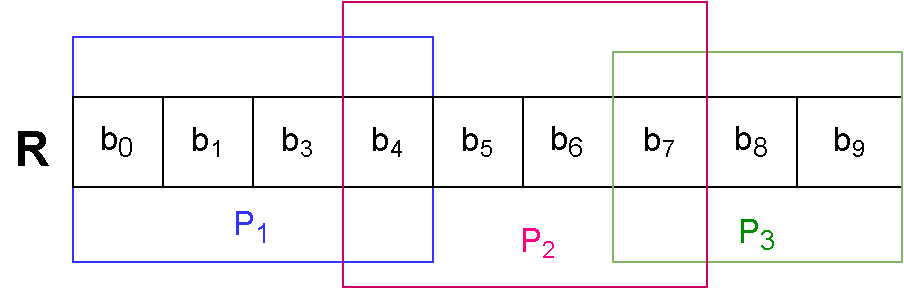
\includegraphics[width=9cm]{JournalDecPulvMod.pdf} 
\caption{Decomposition of row $R$ to $3$ parts} 
\label{fig:decompositionPulv}
\end{center}
\end{figure} 


\textbf{Generating sub-models}. Using the $PTA\_PSP$ model for UPPAAL-CORA, the generation of the sub-models for each row part consists only in editing the input data of the model. No change is needed in the description of the automata. The global constants describing commands are updated with information related to the corresponding row part: the value of the number of blocks forming the row is replaced with the value of the number of blocks forming the part (constant \texttt{nb$\_$block}); and all the tables storing the information of these blocks will be updated with only the concerned blocks. % (typically $ Cbest[]$, $ CAlt[]$, $ tempo\_bloc[] $ and $ Choice[] $). 
It is worth noting that, as the configuration of the models is based on text files, the modelling decomposition can easily be automated.

\Olivier{MARQUE PROGRESSION}

\subsection{Verification Decomposition}
\label{VD}
The verification decomposition decomposes the resolution of the property to be checked on the global model into the resolution of properties on the sub-models.

Let us recall that the property allowing to obtain the optimal command sequence applied on all the rows is the property \texttt{PP3} 
described in the section \ref{sec:VerifProp}. The verification process on the sub-models is based on the same property, but with the modifications of the models previously mentioned. %\footnote {We recall that $ currentBlock $ is the current block that the sprayer is spraying and $ nb \_block $ is the number of blocks forming the row.}:
%\[
%\big( E <> currentBlock == nb \_block-1\big) \ and \ StartRowAut.end
%\]
%The optimal command sequence selects for each block a command between $ C_{best} $ or $ C_{alt} $ while minimising the quantity of product necessary to treat all the row and while ensuring a sufficient protection for each block.
%\vskip 0,2 cm
The decomposition of the verification consists in verifying this property on each row part. It is important to note that in the model of a part, $ nb\_block $ becomes the number of blocks forming the part and $ StartRowAut.end $ is reached when the sprayer finishes spraying all the blocks of the part. 

Checking the property \texttt{PP3} %\ref{reqPulv} 
on the sub-model allows to calculate the Optimal Sequence $ SO_ {i} $ to be applied on the part $ Pi $ and to calculate its Optimal Cost $ CO_{i} $. 
As described in equations (\ref{eq:SOSOi_m}) and (\ref{eq:COCOi_m}), the complete optimal sequence can be calculated from the union of the optimal sequences of the parts $ SO_ {i} $, and the global optimal cost can be calculated from the sum of the optimal costs of the parts $ CO_{i} $, with rectification terms that will be explicited for the case at hand hereafter. 

%This will be proved in the next section.


\subsection{Decomposition Analysis}
\label{PreveComp}

The decomposition analysis proves that the verification of the properties on the sub-models allows the verification of the initial property on the global model. In a decomposition case without overlapping, i.e  the equations (\ref{eq:SOSOi}) and (\ref{eq:COCOi}) are to be proved true. In the case of overlapping, rectification terms $ocr$ and $dcr$ are to be defined and justified and equations (\ref{eq:SOSOi_m}) and (\ref{eq:COCOi_m}) should hold.
\vskip 0,2 cm
Some supplementary formal notations are required.
%STOP RIM  

\subsubsection{Formal definitions}

\paragraph{\textbf{Formal definitions for a row.}} 
Let:
\begin{itemize}
\item $m$ be the number of blocks in the row $R$,
\item $cmd_k$ be the chosen command in the optimal sequence for the block $k$,
\item $co_k$ be the cost corresponding to $cmd_k$. 
%It can be decomposed, as was done in the section \ref{step1}, for $k \in \{1, m\}$:
As was explained with an example in section \ref{sec:InterestCalt} %\ref{step1} 
this cost can be decomposed into three types of local cost: the cost for the spraying required in block $k$, and the supplementary costs required for respectively closing nozzles used at block $k-1$ unused at $k$ and opening nozzles unused at $k$ and used at $k+1$.

Local costs for $k \in \{1, m\}$ can thus be defined as:
\begin{equation}\label{COK}
co_k = Close_k(cmd_{k-1}) + b_k(cmd_k) + Open_k(cmd_{k+1})  
\end{equation}
%\Karen{XXXXXXX Simplification possible : }
%\begin{equation}\label{COK}
%\Karen{co_k = Close_k + b_k + Open_k}  
%\end{equation}
%\Karen{XXXXXXXXXXXXXX }

with :
\begin{itemize} 
\item $X$, $Close(X)$, $Open(X)$ and $b_k(X)$ defined as in section~\ref{sec:InterestCalt}% $X$ is a sprayer nozzle : $X \in \{LH, CH, HH\}$,
\item
% DIT PLUS HAUT $Close_k(cmd_{k-1})$ is the amount of product sprayed, at the beginning of the block $ k $, for closing nozzles which are involved in the command $cmd_{k-1}$ of the previous block but not involved in the command $cmd_{k}$ of block $k$.
For the first block, no command is involved in the previous block which is undefined. In this case, $Close_1()=0$. Otherwise the mathematical formulation of this cost results from its definition:
%$$Close_k(cmd_{k-1}) = \sum\limits_{X \in cmd_{k-1} \wedge X \notin cmd_{k}} Close(X)$$
\begin{align}
\text{for } k \in \{2,m\}, &  \quad Close_k(cmd_{k-1}) = \sum\limits_{X \in cmd_{k-1} \wedge X \notin cmd_{k}} Close(X) \nonumber \\
 \text{else} & \quad Close_1()=0  \label{eq:CloseNul}
\end{align}

\item $b_k(cmd_k)$ is the amount of product sprayed by nozzles involved in the command $cmd_k$ chosen for the block $k$: 
$$b_k(cmd_k) = \sum\limits_{X \in cmd_k} b_k(X)$$
\item $Open_k(cmd_{k+1})$ has a similar construction.
%is the amount of product sprayed, at the end of the block $ k $, for opening nozzles which are involved in the command $cmd_{k+1}$ of the next block but not involved in the command $cmd_{k}$ of block $k$.
For the last block, no command is involved in the (undefined) next block. In this case, $Open_m()=0$.
%$$Open_k(cmd_{k+1}) = \sum\limits_{X \notin cmd_k \wedge X \in cmd_{k+1}} Open(X)$$
%\Karen{XXXX A RAJOUTER : $Open_n()=0$ for the last block of the row XXXX}
\begin{align}
\text{for } k \in \{1,m-1\}, &  \quad Open_k(cmd_{k+1}) = \sum\limits_{X \notin cmd_k \wedge X \in cmd_{k+1}} Open(X) \nonumber \\
 \text{else} & \quad Open_m()=0 \label{eq:OpenNul}
\end{align}
\end{itemize}

\item $co_{init}$ be the amount of product sprayed for opening nozzles which are required in the command $cmd_1$ for the first block and $co_{end}$ the amount of product sprayed for closing nozzles which are used in the last block :
%\begin{eqnarray*}
%co_{init} & = & \sout{Open(cmd_1)}\ \ = \sum\limits_{X \in cmd_1} Open(X) \\
% co_{end} & = & \sout{Close(cmd_{m})} = \sum\limits_{X \in cmd_m} Close(X)
%\end{eqnarray*}
%\Karen{\textbf{XXXXXXX PROPOSITION KAREN}}
\begin{eqnarray*}
co_{init} & = & \Karen{Open_{init}(cmd_1)}\ \ = \sum\limits_{X \in cmd_1} Open(X) \\
 co_{end} & = & \Karen{Close_{end}(cmd_{m})} = \sum\limits_{X \in cmd_m} Close(X)
\end{eqnarray*}

\item  The Optimal Sequence $SO_R$ applied on the row $R$ can be written:
\begin{equation}
    SO_R  = \overset{m}{\underset{k=1}{\bigcup}} cmd_k  \label{eq:SOR}
\end{equation}
%$$SO = \overset{m}{\underset{k=1}{\bigcup}} cmd_k $$
\item  The Optimal Cost $CO_R$ in quantity of sprayed product for the row $R$ can be written:
\begin{equation}
    CO_R  = co_{init} + \overset{m}{\underset{k=1}{\sum}} co_k + co_{end}  \label{eq:COR}
\end{equation}
%$$CO  = co_{init} + \overset{m}{\underset{k=1}{\sum}} co_k + co_{end}$$
\end{itemize}


\vskip 0,1 cm
\paragraph{\textbf{Formal definitions for a part.}} 

The row $R$ is divided into $ n $ parts $ P1 $, ..., $Pn $.  The notations defined for a whole row can be extended to a part $ Pi $:% Let:
\begin{itemize}
\item $l_{i}$ is the number of blocks in the part $Pi$.
\item all of the above definitions must be stated in relation to the parts: $cmd_{k}$ becomes $cmd_{i,k}$, $Close_k$ becomes $Close_{i,k}$, etc.
%\item $cmd_{i,k}$ be the chosen command for the block $k$ in the part $Pi$. 
%\item $co_{i,k}$ be the cost corresponding to $cmd_{i,k}$ %(including initial and final costs)
\item $SO_{i}$ is the optimal sequence applied on the part $Pi$ :
\begin{equation}
    SO_{i} = \overset{l_{i}}{\underset{k=1}{\bigcup}} cmd_{i,k} \label{eq:SOi}
\end{equation}
%\[SO_{i} = \overset{l_{i} - 1}{\underset{k=0}{\bigcup}} cmd_{i,k} \]
\item $CO_{i}$ is the optimal cost in quantity of sprayed product for the part $Pi$ :
\begin{equation}
    CO_i  = co_{i,init} + \overset{l_i}{\underset{k=1}{\sum}} co_{i,k} + co_{i,end} \label{eq:COi}
\end{equation}
\end{itemize}


\subsubsection{Proof of the optimal sequence and cost conservation} 


% DEJA DIT The goal of the proof is now to show that equation (\ref{eq:SOSOi}) and (\ref{eq:COCOi}) given section \ref{sec:DecompoConcept} are true, i.e. to prove that the optimal cost $CO_R$ (resp. the optimal command sequence $SO_R$) directly obtain in the whole row R is the same as the sum of the optimal costs of the $CO_i$ (resp. the union of the optimal command sequences $SO_i$) calculated in the parts of the row.

The proof will be illustrated on a row composed of 5 blocks, named $b_1$ to $ b_5 $, as shown in figure~\ref{fig:decompoo}. The duration of each block is greater than the sum of the opening and closing times of the nozzles, which is a necessary assumption given in the step 2 of AMPS. The row is divided into 2 parts: $ P1 $ groups together the first three blocks, and $ P2 $ includes the blocks $ b_3 $ to $ b_5 $. $b_{3}$ is the overlapping block and so is included in both P1 and P2.


\begin{figure}[h!]
\begin{center}
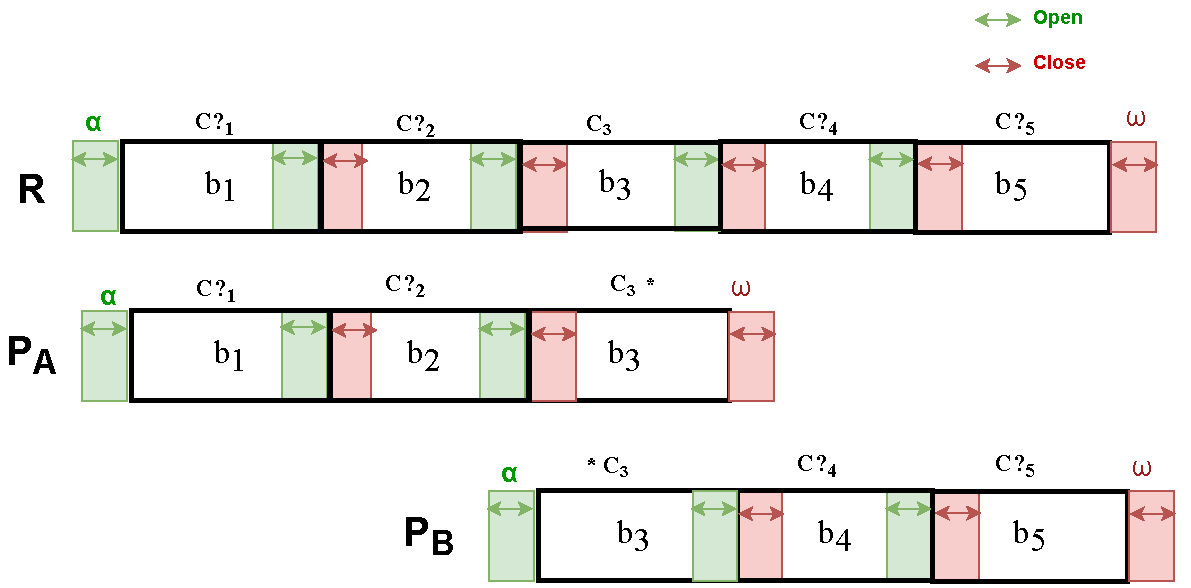
\includegraphics[width=12cm]{decompo2.pdf} 
\caption{Illustration of the proof of decomposition} 
\label{fig:decompoo}
\end{center}
\end{figure} 



%To prove that the decomposition method guarantees the conservation of the verification and spray optimization property (Property \ref{reqPulv})
In the following, it will be shown that the decomposition keeps consistency between the optimal cost for the whole row and optimal costs for the parts, as well as for the optimal command sequences.

%we will compare and analyze the verification results of the property \ref{reqPulv} applied in the initial row and in the decomposed row. 



\paragraph{\textbf{Optimal command sequence and cost of the example row R.}} $ \\ $

For the example row $R$, the optimal sequence applied is (equation~\ref{eq:SOR}):
\begin{equation}
SO_R = cmd_{1} \cup cmd_{2} \cup cmd_{3} \cup cmd_{4} \cup cmd_{5}  \label{eq:SORExample}
\end{equation}
and the optimal cost is (equation~\ref{eq:COR}) :
\begin{equation}
CO_R = co_{init}+co_{1}+co_{2}+co_{3}+co_{4}+co_{5}+co_{end} \label{eq:CORExample}
\end{equation}

\indent As $b_{3}$ is the overlapping block, it is useful to detail its cost using equation \ref{COK}:
\begin{equation}
co_3 = Close_3(cmd_{2}) + b_3(cmd_3) + Open_3(cmd_{4})  \label{eq:co3} 
\end{equation}

\paragraph{\textbf{Equivalence of the optimal sequences.}} $ \\ $

As explained in section~\ref{sec:AMPSmethodo} and illustrated in figure~\ref{fig:CbestCalt}, the choice of the optimal sequence of a block depends on 1) the PSM function which defines the $C_{best}$ and $C_{alt}$ choices for this block, and 2) the possible commands of the previous and the next blocks. Thus, it is not possible to suppress $b_3$ from one of the part: both the optimal commands of $b_2$ and $b_4$ depend on the command of $b_3$. Overlapping is necessary with this decomposition criterion.  
Considering this overlapping, it can be assured that the optimal commands chosen for each of the blocks is the same in the complete row than in both parts.
% INUTILE \footnote{We supposed that the block ID, i.e. their number, does not change: $b_3$ remains $b_3$ even when it is the first block of the part $P_2$.}:
\begin{equation}
    \forall k, \forall i, \ cmd_{k}=cmd_{i,k} \label{eq:cmdikcmdk}
\end{equation}


Considering that the overlapping block $b_3$ is present in both the parts, the union of $SO_{1}$ and $SO_{2}$ will include 2 $cmd_{3}$ ($cmd_{1,3}$ and $cmd_{2,3}$) while this command will be applied only once for the spraying of the whole row. The $ocr$ term of equation \ref{eq:SOSOi_m} can be identified as:
\begin{equation*}
    ocr = cmd_{3}
\end{equation*}

Identifying $SO_R$ as $SO$ for the illustrative example, equation \ref{eq:SOSOi_m} holds.


\paragraph{\textbf{Equivalence of the optimal costs.}} $ \\ $

The overlapping block $b_3$ in our example introduces additional costs that do not apply when spraying and identified as $dcr$ in \label{eq:COCOi_m}. As shown in figure \ref{fig:decompo}, $dcr$ should include the cost of the extra $b_3$ command ($cmd_3$) from the total. It should also include the cost produced by the intermediate closing of the nozzles at the end of $P_1$ and the (resp. beginning) of the part, which are virtual additional costs added by the decomposition. In reality, the nozzles will not be closed after $b_3$ as the sprayer will treat the row as a whole.

So, with $CO_D$ the optimal cost of the decomposed row calculated from the parts, we have:
\begin{eqnarray}
CO_D &=& CO_1 + CO_2 - co_{1,end} - co_{2,init} - b_{3}(cmd_3)  \label{preuveDecompo_cout}
\end{eqnarray}

Now we want to prove that $CO_D$ is equal to the global cost $CO_R$. We first focus on the cost of the part $P1$. As the overlapping block $b_3$ is the last block in $P1$, we have $Close_{1,3}=0$ \Rim{$Open_{1,3}()=0$} (equation~\ref{eq:CloseNul}) and:

$$co_{1,3} = Close_3(cmd_{1,2}) + b_3(cmd_{1,3})$$
\Rim{$$co_{1,3} = Close_{1,3}(cmd_{1,2}) + b_3(cmd_{1,3})$$}
For the whole part $P1$, we must consider the additional cost $co_{1,end}$ necessary to virtually close the nozzles after $b_3$. Considering equations \ref{eq:COi}, \ref{eq:cmdikcmdk} and the previous one, we have :

\begin{eqnarray}
CO_1 & = & co_{1,init}+co_{1,1}+co_{1,2}+ co_{1,3}+ co_{1,end}  \nonumber\\
CO_1 & = & co_{init}+co_{1}+co_{2}+Close_3(cmd_{2}) + b_3(cmd_{3})+ co_{1,end} \label{eq:CO1Exemple}
\end{eqnarray} 

In the same way, as $b_3$ is the first block in $P2$, we establish that:

\begin{eqnarray}
CO_2 & = & co_{2,init}+co_{2,3}+co_{2,4}+co_{2,5}+co_{2,end}  \nonumber\\
CO_2 & = & co_{2,init}+b_3(cmd_{3}) + Open_3(cmd_{4})+co_{4}+co_{5}+co_{end}  \label{eq:CO2Exemple}
\end{eqnarray}


Calculating the optimal cost $CO_D$ for the row formed by $P1$ and $P2$ with the equation \ref{preuveDecompo_cout}, and using the equations \ref{eq:CO1Exemple}, \ref{eq:CO2Exemple}, \ref{eq:CORExample} and \ref{eq:co3}, we can prove the equality of the optimal costs: 
\begin{eqnarray*}
CO_D &=&co_{init}+co_{1}+co_{2}+Close_3(cmd_{2}) + b_3(cmd_{3})+ co_{1,end} \nonumber\\
&& +\ co_{2,init}+b_3(cmd_{3}) + Open_3(cmd_{4})+co_{4}+co_{5}+co_{end} \nonumber\\
&& -\ co_{2,init} - b_{3}(cmd_{3}) - co_{1,end} \nonumber\\
CO_D &=&co_{init}+co_{1}+co_{2}+Close_3(cmd_{2}) + b_3(cmd_{3}) + Open_3(cmd_{4})\nonumber\\
&&  +co_{4}+co_{5}+co_{end}  \nonumber\\
CO_D &=&CO_R 
\end{eqnarray*}



\vskip 0,3 cm


Thus we have proved that the optimal cost and the optimal command sequence are the same for the initial and the decomposed rows. We illustrate it on a specific example, but this proof is applicable regardless of the number of parts in the row. Thus, our decomposition method is proved for the criterion $C_{best}=C_{alt}$. This proof is also applicable for the other criteria, in a more simple way. For example, if we decompose using hole of vegetation, the spraying product used in the overlapping block is nil, and the proof remains valid.

In the next section, the decomposition methodology is applied on a real vine plot.

%XXXXXXXXXXXXXXXXXXXXXXXX KAREN : FIN RELECTURE XXXXXXXXXXXXXXX
